%% The following is a directive for TeXShop to indicate the main file
%%!TEX root = diss.tex

\chapter{Entropy in mesoscopic systems}
\label{ch:Theory}

In this chapter, we review the theoretical underpinnings for the measurements that were completed. First, we discuss some of the theory behind single and double quantum dots and the relevant energy scales for these systems. We then proceed to a review of entropy in quantum systems, finally discussing the Maxwell relation used to make the measurements of entropy presented in this thesis and those presented by Hartman et al.

\section{Entropy of quantum systems}
The classical description of entropy comes in the form of the Boltzmann entropy
\begin{equation}
	\label{eqn:b_entropy}
	S = k_b \ln W.
\end{equation}
Here, $W$ is defined by the number of available microstates of the system \cite{schroeder}. In the context of simple quantum systems at $T$ close to zero (such that excited states are unattainable), it is useful to consider this quantity, $W$, as the degeneracy, $d$, of the ground state of the system~\cite{mcquarrie}. 

As a simple example, and closely related to the results from this thesis, consider a single potential well that may be occupied by some small number of electrons as illustrated in Fig~\ref{fig:potential_wells} (a).  In the example outlined Fig~\ref{fig:potential_wells} (a), the possible occupations, $n$, of the well are shown. This system can also be thought of, very approximately, as a model for a single atom with excited states unreachable at low enough $T$~\footnote{In practice, potential wells like this can be fabricated on a mesoscopic scale -- much larger than any atom -- to study the behavior of electrons in ``artificial" atoms cf. Ch. ~\ref{ch:Methods}.}. In the $n = 0$ state the system has no degeneracy since there is only one state at ground state energy -- no electrons anywhere. However, in the $n=1$ state, the system develops a ground state degeneracy of $d = 2$ since the single electron will be in either a spin up or spin down state, both of which will be of the same energy. Finally, if a second electron is added to the system, the spin degeneracy of the system will break as the lowest energy state of the pair of electrons will be a spin singlet state disallowing net spin freedom of the system. 

One can consider the change in entropy, $\Delta S$, of a given transition in the occupation of the quantum dot\footnote{For now, where this electron came from will be neglected.} like the transition from $n = 0 \to n = 1$ as shown in Fig~\ref{fig:potential_wells} (b). For this transition, $\Delta S = k_B \ln d_f - k_B \ln d_i = k_B \ln 2$ by Eqn.~\ref{eqn:b_entropy}.
\begin{figure}[h]
\centering
\resizebox{1\textwidth}{!}{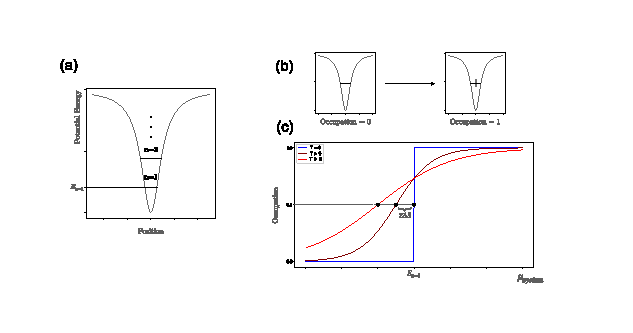
\includegraphics{figures/pdfs/quantum_well_theory.eps}}
\caption{In (a) a simple potential well is shown, with the energy levels of various occupations plotted on top of the potential diagram. In (b) and (c) a transition from $0 \to 1$ electrons in the potential well is illustrated. In (c) finite temperature broadening of this transition, as well as a shift in $\mu_{system}$, due to the change in entropy of the transition, is shown as temperature increases (still much too small to allow for excited states). }
\label{fig:potential_wells}       % Give a unique label to the figure. 
\end{figure}

Next, we consider the energy at which such a transition would occur, labelled as $E_{n=1}$ for $T=0$. As temperature is increased, the chemical potential of the system, $\mu_{system}$, at the ``half-occupancy" point of such a transition will be affected by the $\Delta S$ of the system due to the effect that entropy has on the Helmoltz free energy, $F$, of a given configuration.
\begin{equation}
	F = E - T \Delta S \quad \to \quad \mu_{sys, transition}  = E_{n=1} - T \Delta S
\end{equation}
Graphically, this effect is shown in Fig~\ref{fig:potential_wells} (c), where in addition to an effective broadening of the transition from finite $T$, the ``half-occupancy" point of the transition from $0 \to 1$ electrons shifts in $\mu_{system}$. It is this affect which we have used in measurements in this thesis to quantify changes in entropy.

\section{From a Maxwell relation to entropy}
\label{sec:mrtoentropy}

The shift in the transition based on a change in entropy as summarized above can be quantified by the following Maxwell relation.

\begin{equation}
	\label{eqn:MR}
	\left( \frac{\partial \mu }{\partial T} \right)_{p,N} = -\left( \frac{\partial S}{\partial N} \right)_{p,T}
	%\Delta S = \int_{\mu_1}^{\mu_2} \frac{dN(\mu)}{dT}\,\, d\mu
\end{equation}


In other words, by measuring the occupation of a quantum dot as a function of the chemical potential, $N(\mu)$, and varying temperature, $T$, we can derive the change in entropy, $\Delta S$ over that change in occupation.

In systems with few degrees of freedom, the relevant discussion of entropy comes in the form of Boltzmann entropy, $S = k_b \ln \Omega$ with $\Omega$ being the number of available microstates~\cite{schroeder}. In Hartman et al.'s experiment, it was shown that the change in entropy as a quantum dot goes from an occupation of $0 \to 1$ electrons was $\Delta S = k_b \ln 2 - k_b \ln 1 = k_b \ln 2$ as the dot went from only having one possible state to having two possible spin states (spin up and spin down). In addition, it was shown that by applying a large magnetic field, Zeeman splitting of the energy levels in the dot eliminated this degeneracy causing $\Delta S = k_b \ln 1 - k_b \ln 1 = 0$.

In practice, to measure the entropy of a small system using a mesoscopic circuit and the integral from Eqn.~\ref{eqn:MR} we have a few requirements. First, we assumed constant pressure in the Maxwell relation. In the context of a 2-dimensional electron gas (2DEG) with which our measurements are conducted, the dominating pressure at temperatures below the Fermi temperature, $T_F \approx 100$K is the degeneracy pressure~\cite{ashcroftmermin}, an incompressibility emerging from the Pauli exclusion principle disallowing fermions from occupying the same quantum state. In addition, by keeping energy fluctuations due to thermal energy, $k_bT$, much smaller than the spacing between energy levels in the dot, we ensure that random temperature fluctuations do not produce unpredictable energy level occupation.
To carry out the integration from Eqn.~\ref{eqn:eqn1} in practice, it is necessary to have an accurate way of measuring the occupancy, $N$, of the probe dot. We measure $N$ by measuring the conductance $G_{sens}$ through a charge sensing quantum point contact (QPC) seen in Fig.~\ref{fig:device}. 

Because of the proximity of this QPC, referred to as the charge sensor, to the probe dot very small electrostatic changes in the probe dot affect the conduction across the charge sensor~\cite{spintocharge}. As such, a larger $G_{sens}$ indicates fewer electrons in the probe dot, while a smaller $G_{sens}$ indicates more electrons in the probe dot. In effect, this means that $G_{sens}$ can be used to directly measure the occupancy of the dot as a function of various other quantities like chemical potential, $\mu$, or temperature, $T$. We use $V_{plunger}$ ($V_p$) shown in in Fig.~\ref{fig:device} to locally control the chemical potential of the dot. Varying the potential applied to this gate $V_p$ - and by extension the chemical potential in the dot - is our primary technique to control the occupancy of the dot. Based on this protocol, we can decompose Eqn.~\ref{eqn:eqn1} into the following quantities which can be determined experimentally.
\begin{equation}
	\label{eqn:eqn2}
	\Delta S = \int_{\mu_1}^{\mu_2} d G_{sens}\frac{dN}{dG_{sens}} \frac{1}{dT} \,\,  d \mu
\end{equation}
This integral tells us that we can measure the change in entropy between two chemical potentials in the dot by measuring three quantities: $dN/dG_{sens}$, $dT$, and $dG_{sens}$ as a function of chemical potential. The first two quantities $dN/dG_{sens}$ and $dT$ are scaling factors that can be independently experimentally determined but do not depend on $\mu$ however the final quantity $dG_{sens}$ does depend on $\mu$ and so must be measured as $\mu$ is changed. Intuitively, $dG_{sens}$ is a measure of the difference between the occupancy of the dot at higher $T$ and lower $T$ - this is illustrated by the shading on the plots in Fig.~\ref{fig:num_int}. 


\begin{figure}[h]
\centering
\resizebox{1\textwidth}{!}{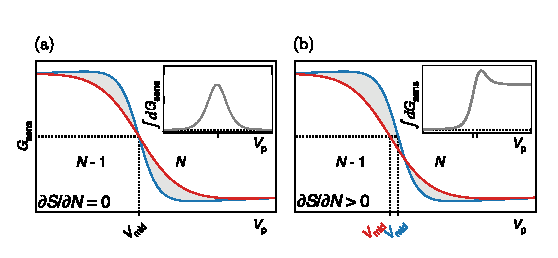
\includegraphics{figures/pdfs/numerical_integrated.eps}}
\caption{ In (a) and (b) we show two examples of the measurement protocol where the occupancy of the probe dot is measured using $G_{sens}$. In each case, the occupancy is swept from $N - 1$ to $N$ electrons both at a higher temperature (red) and a lower temperature (blue), however in (a) this change in $N$ does not correspond to an entropy change in the system whereas in (b) we see a positive change in entropy of the system due to this change in occupancy. The inlaid plots show the cumulative integral of $d G_{sens}$ -- or the difference between hot and cold $G_{sens}$ curves. The entropy change of the system is measured by the value of this integral after the completion of this transition. $V_{mid}$ is labelled for each curve, notably, $V_{mid}$ is the same in the zero entropy case, but shifts in the finite entropy case. Figure from Hartman et al.}
\label{fig:num_int}       % Give a unique label to the figure. 
\end{figure}

Using $V_{degeneracy}$ ($V_d$) the quantum system composed of the two dots (highlighted in yellow in Fig.~\ref{fig:device}) with a single electron confined within the system can be tuned between non-degenerate and doubly-degenerate. This works by first suppressing spin degrees of freedom with a large magnetic field then slowly changing the shape of the potential function separating the two dots using $V_d$. Once the potential barrier between the dots is large enough, the tunneling rate will become negligible.

Capacitive coupling between the probe dot and the pair of dots can be tuned such that occupation of the probe dot suppresses the degeneracy of the two-dot system. This is because the lowest energy state will occur when the two electrons are farthest apart. Thus, we can tune the system to a state where there is an entropy change of the entire thermodynamic system independent (while no change in entropy of the probe dot itself) as the probe dot changes occupation. In this way, we will be able to detect a non zero value of entropy if we are able to detect changes in entropy of a capacitively coupled system. Specifically, by tuning the upper two dot system between non-degenerate and doubly degenerate, we will be able to see the change as entropy as the probe dot transitions $0 \to 1$ electrons vary from $\Delta S = 0$ to $\Delta S = -\ln2$, respectively.



\section{Free energy explanation}
\label{sec:fenergy}

To get a physical intuition for the thermodynamics at work to make this measurement possible, it may be useful to consider the Maxwell relation in Eqn.\ref{eqn:MR} in terms of free energy of the system. More will be added here, specifically, a more complete explanation of the measurement in terms of free energy.

\endinput

Any text after an \endinput is ignored.
You could put scraps here or things in progress.
